\section{Text Analysis and Natural Language Processing: A Diachronic Newspaper Corpus}

Most of the data in the field of crime analysis is unstructured text data, such as police reports and court documents. Last year I focused on the development of a search engine for this kind of documents, facilitating information retrieval for the Prosecutor's Office of Palermo, that is now in use in their daily activities.

However, as the access of most of these documents is restricted, this year I focused on the corpus of all the \textbf{newspaper articles} published by \textit{La Repubblica} between 1985 and 2000, that I built by reverse engineering the CD-ROMs published by the newspaper in the early 2000s.

The dataset is formed by about \textbf{600,000} full-text articles, with metadata like the title, the date of the publication and the author. The corpus was further augmented by scraping the online archive of \textit{La Repubblica} for the section labels for more than 80\% of the articles. It's a particulary interesting set of documents, as it's very generalist and covers one of the most interesting periods in Italian history: the years of the Mafia wars, the fall of Soviet Union, the Tangentopoli corruption scandal and the beginning of the so-called \textit{Second Republic}.

Most of the analysis on the corpus was done during my visiting period at the \textit{Institute for Cross-Disciplinary Physics and Complex Systems} (IFISC) in Palma de Mallorca, Spain, where I worked from March to July 2025 under the supervision of Prof. David Sanchez.

I carried out two main projects: on one side I focused on building a \textit{topic model}, trying to understand which metodologies are best suited to \textit{label} the documents in a unsupervised way. On the other side, I used the diachronic nature of the corpus to analyze the lexical and semantic evolution over time.

From a practical standpoint, the first thing to do is preprocessing and cleaning, which involves splitting the text in words (\textit{tokenization}), removing stop words, and normalizing the text (e.g., lowercasing, stemming, lemmatization). After this step the text is converted into a vector representation, which can be sparse and word-count based (the \textit{TF-IDF} representation, which is a document-term matrix which captures the importance of words in each document) or dense and context-based (using \textit{embeddings}). A dimensionality reduction step is often applied, usually via \textit{PCA} or \textit{UMAP}. The result is a set of vectors in a lower-dimensional space that can be used for further analysis. In the case of topic modeling, clustering algorithms like \textit{K-Means} and \textit{HDBSCAN} group together similar documents.

One of the most interesting results came from the dynamical analysis: by splitting the documents by month I was able to build \textit{time series} of words importance (using TF-IDF scores) and of "\textit{media discourse}" (the center of mass of the document vectors in each month). The former can be seen as a \textit{lexical} analysis, while the latter is more \textit{semantic} in nature.

More specifically, the media discourse is computed as
\begin{equation}
    \vec{c}\,(m) = \frac{1}{N_m} \sum_{i = 1}^{N_m} \vec{d}\,_i^{(m)}
\end{equation}
where $N_m$ is the number of documents in month $m$ and $\vec{d}\,_i^{(m)}$ is the vector representation of document $i$ in month $m$. The document vectors were obtained by applying \textit{PCA} on the TF-IDF representation, keeping the first 100 components.

These time series show patterns that are consistent with the major historical changes in Italy. For example, by computing a \textit{cosine similarity matrix} (see \autoref{fig:sim_mat}) between the media discourse vectors of each month I was able to identify the Gulf War in 1991, the Kosovo War in 1999, and the beginning of the Second Republic in 1994.

%On the other hand, by estimating the Shannon entropy from the eigenvalue specrum of the covariance matrix of the documents in each month, I could identify periods of higher and lower diversity: in particular, the periods of the Gulf War and of the Kosovo War show a more focused discourse, and a lower entropy (\autoref{fig:shannon_entropy}).

\begin{SCfigure}[][ht]
    \centering
    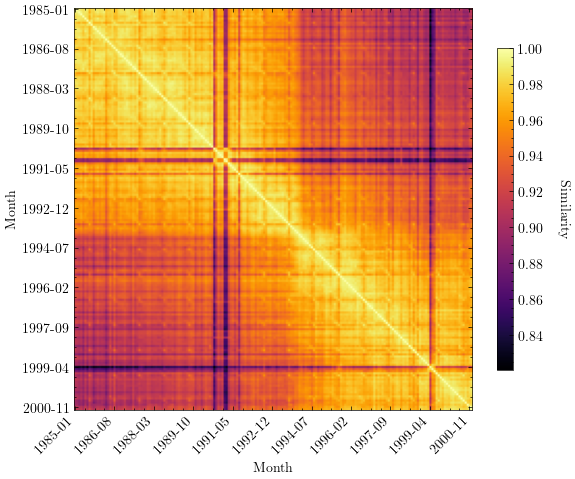
\includegraphics[width=0.5\textwidth]{figures/sim_mat.png}
    \caption{
        Cosine similarity matrix of semantic center of mass (1985-2000). 
        Darker colors indicate greater semantic change. 
        The block-diagonal structure reveals temporally coherent discourse regimes and transitions aligned with major historical events: the transition from the First to the Second Republic in 1994, the Gulf War in 1990-1991, and the Kosovo War in 1999.
    }
    \label{fig:sim_mat}
\end{SCfigure}

The techniques are very general and can be applied on other corpora, for example on the documents in the Prosecutor's Office archive. Such an approach could provide not only a useful tool for easier navigation of the documents, but also a way of defining "periods" in Mafia history based on the actual discourse, giving a quantative complement to the qualitative analysis usually done by historians and criminologists.
